\documentclass[a4paper,12pt]{article}

\usepackage[T1]{fontenc}
\usepackage[utf8]{inputenc}
\usepackage{lmodern}
\usepackage[english]{babel}

% math symbols
\usepackage{amsmath}
\usepackage{amssymb}

% nice looking tables
\usepackage{booktabs}
% columns spanning over multiple cells
\usepackage{multicol}

% sub floats for figures and tables
\usepackage{subcaption}
\usepackage[font=small,labelfont=bf]{caption}

% set smaller margins
\usepackage[margin=2cm]{geometry}
% don't allow to go far past the margin
\setlength{\emergencystretch}{2em}
% enable margin kerning and font expansion (for better spacing)
\usepackage[protrusion=true,expansion=true]{microtype}

% extra space between paragraphs
\setlength{\parindent}{0pt}
\setlength{\parskip}{1ex plus 0.5ex minus 0.5ex}

% penalise orphans and widows
\widowpenalty=10000
\clubpenalty=10000

% clickable urls
\usepackage{url}

% references and coloured hyperlinks
\usepackage{hyperref}
\hypersetup{pdfborder=0 0 0,colorlinks=true,bookmarksnumbered,urlcolor=magenta,plainpages=false}

% import vector images and bitmaps from a predefined path
\usepackage{graphicx}
\DeclareGraphicsExtensions{.pdf,.png,.jpg}
\graphicspath{ {figures/} }

% standard colour names
\usepackage[svgnames]{xcolor}


% metadata
\title{CSC3432 report}
\author{Kristen Karsburg Arguello}
\date{December 2024}

\begin{document}

\maketitle

\section{Task 1 - Network Visualization}

\newcommand{\threshold}{50\% } 
% need to figure out an explanation for the 50% score


\subsection{Methods}
\begin{enumerate}
    \item Decompress the sequences file, split it into lines, and remove empty ones.
    \item Set up the BioPython pairwise aligner with gap penalties of -10 and -0.5, use the BLOSUM-62 matrix, and set the mode to 'local', as exemplified in the module documentation.
    \item For each sequence, compute alignment scores with others, normalize by the longest sequence length, as longer sequences have more opportunities for combinations, while shorter sequences may be more similar but have fewer opportunities for string matches, and store it in a zero-filled matrix. 
    \item Set a threshold based on score distribution (\threshold of max similarity) and create a graph with nodes as sequences and edges for scores above the threshold.
    \item Use a community detection algorithm like Infomap, colour nodes by cluster, scale by degree, and plot the graph as in Figure \ref{fig:network-1}.
    \item Create a table of the network's topological attributes, as in Table \ref{tab:topological-network-1}, to identify clusters.
\end{enumerate}


\begin{figure}[h]
  \centering
  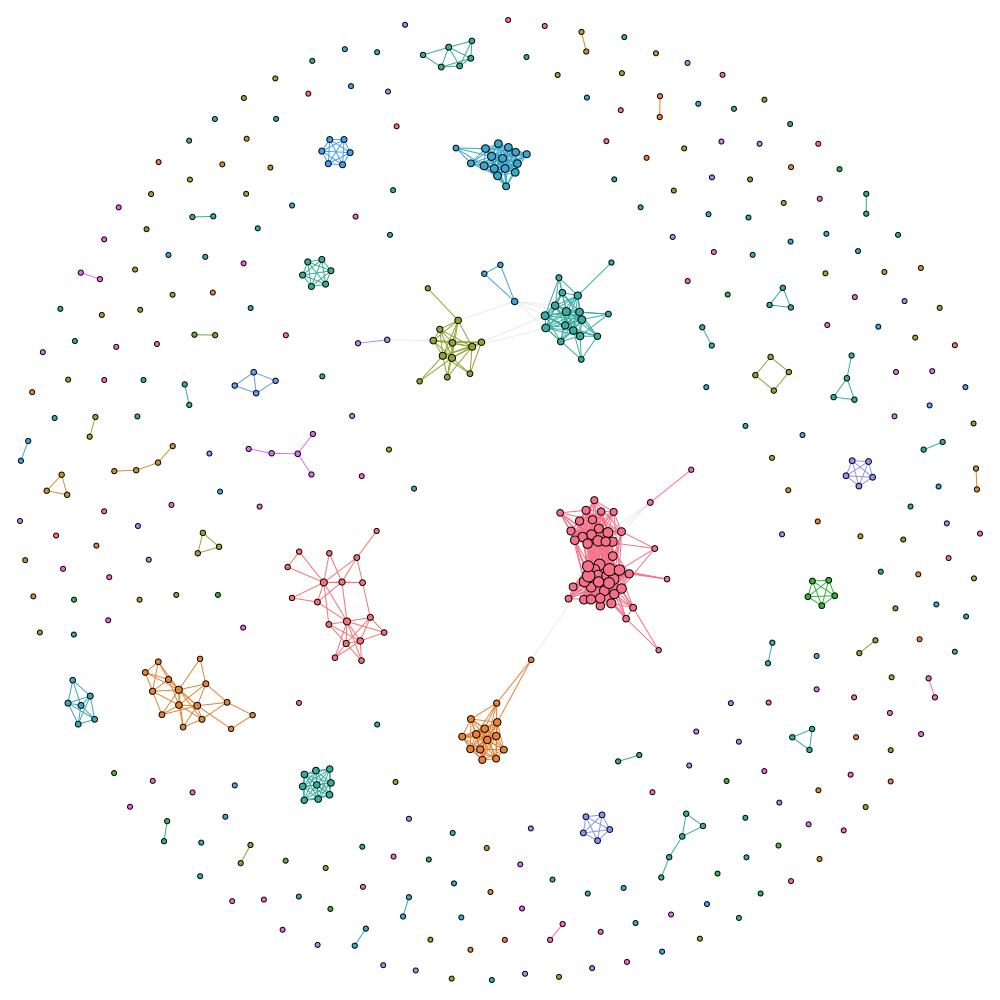
\includegraphics[width=300px]{1_network.png}
  \caption{Visualization of the generated network with the nodes coloured and sized by their cluster memberships and connections.}
  \label{fig:network-1}
\end{figure}


\subsection{Results}
The analysis of protein sequences through pairwise alignment and community detection reveals the presence of distinct clusters of homologous proteins. By employing a threshold, set at \threshold of the maximum similarity score, we can connect proteins that exhibit an above-average similarity. This threshold allows for identifying homologous relationships, where proteins share a common evolutionary ancestor. Adjusting the threshold can yield different clusters; a higher threshold requires proteins to be extremely similar, while a lower threshold can capture more distant homologues.

In the constructed network, seen on Figure \ref{fig:network-1}, clusters are visually represented by nodes of different colours and sizes. These clusters suggest evolutionary relationships, functional similarities, and structural conservation among the proteins. Proteins that do not form clusters are likely to lack strong similarity with others, possibly indicating a lack of common ancestry.

The network's topological attributes, seen on Table \ref{tab:topological-network-1}, such as transitivity, further support the presence of clusters. A high degree of transitivity (over 0.7) suggests that neighbouring nodes are also neighbours, indicating a high level of clustering. This tendency can be attributed to common ancestry, where evolutionary processes lead to the formation of homologous protein clusters. Functional conservation also plays a role, as natural selection preserves sequences with beneficial functions across evolution. Additionally, gene duplication and divergence contribute to homologous clusters, where one gene copy retains the original function while the other undergoes mutations.

Overall, the presence of clusters in the network highlights the evolutionary and functional relationships among protein sequences, providing insights into their shared origins and conserved functionalities.

\begin{table}[h]
\centering 
\begin{tabular}{lr}
\toprule
Metric & Value \\
\midrule
    Diameter & 6 \\
    Girth & 3 \\
    Average Path Length & 2.326 \\
    Average Degree & 3.953 \\
    Assortivity Degree & 0.690 \\
    Transitivity Average & 0.777 \\
    Transitivity Undirected & 0.706 \\
\bottomrule
\end{tabular}
\caption{
    Network topological properties. 
}
\label{tab:topological-network-1}
\end{table}


\pagebreak
\section{Task 2 - simple ML}

\subsection{Methods}
\begin{enumerate}
    \item Load datasets, keep only CDR attributes from the first visit, and left join other visits using patient ID. Remove non-varying, non-patient-related, or identification columns (e.g., visit, MRI delay, patient ID, MRI ID). Fill missing data with the mode, correct CDR typos, and convert nominal (sex, hand) and ordinal categories (CDR levels, SES) to ordered integers.
    \item Add a column indicating if a patient's condition worsened in any of the later visits compared to the first, to aim on preventing worsening at any given point, considering improvements as non-related. 
    \item Split the dataset: 20\% for testing, the rest for training. 
    % TODO: fazer o flow da pipeline
    \item  Create a pipeline with a scaler and logistic regression classifier, as shown in Figure \ref{fig:pipeline-2}. Perform grid search, with the listed values below, with shuffled cross-validation (15 folds) for each regularization type (None, L1, L2), measuring ROC-AUC and F1. 
    \begin{itemize}
        \item No penalization grid: solvers (lbfgs, newton-cg), class-weight (balanced, none), fit-intercept (true, false).
        \item L1 penalization grid: C (0.1 to 1, step 0.1), solver (liblinear), fit-intercept (true, false), intercept scaling (0.1 to 5, step 0.25), class-weight (balanced, none).
        \item L2 penalization grid: C (0.1 to 1, step 0.1), solvers (lbfgs, liblinear, newton-cg, newton-cholesky), class-weight (balanced, none), fit-intercept (true, false).
    \end{itemize}
    \item Calculate mean learning performance with a 95\% confidence interval for each regularization type.
    \item Plot a heatmap of disease progression for each initial condition level and create a table showing dataset value count distribution.
\end{enumerate}

\begin{figure}[h]
  \centering
  \includegraphics[width=200px]{task2.png}
  \caption{Set pipeline as a flow diagram.}
  \label{fig:pipeline-2}
\end{figure}


\subsection{Results}
Predicting dementia worsening after a first visit is challenging, as the model's ROC-AUC scores are only slightly better than random guessing, indicating difficulty in distinguishing between worsening and non-worsening patients. Low F1 scores further highlight the model's struggle to accurately predict the positive class. These metrics suggest that while predictions are possible, they are not reliable or accurate enough for effective use.


A major issue is the dataset imbalance, with only 20\% of patients experiencing worsening, as shown in Table \ref{tab:imbalanced-data-2}. Figure \ref{fig:disease-progression-2} illustrates that most patients remain stable, with few worsening or improving. This imbalance biases the model towards predicting the majority class, leading to poor performance. Techniques like resampling, different evaluation metrics, or algorithms for imbalanced data could improve performance. The grid search identified balanced class weight as the best parameter to mitigate this imbalance.  

\begin{table}[h]
\centering
\begin{tabular}{lr}
\toprule
Worsening & Proportion \\
\midrule
No & 0.79 \\
Yes & 0.21 \\
\bottomrule
\end{tabular}
\caption{
    Dataset distribution.
}
\label{tab:imbalanced-data-2}
\end{table}

\begin{figure}[h]
  \centering
  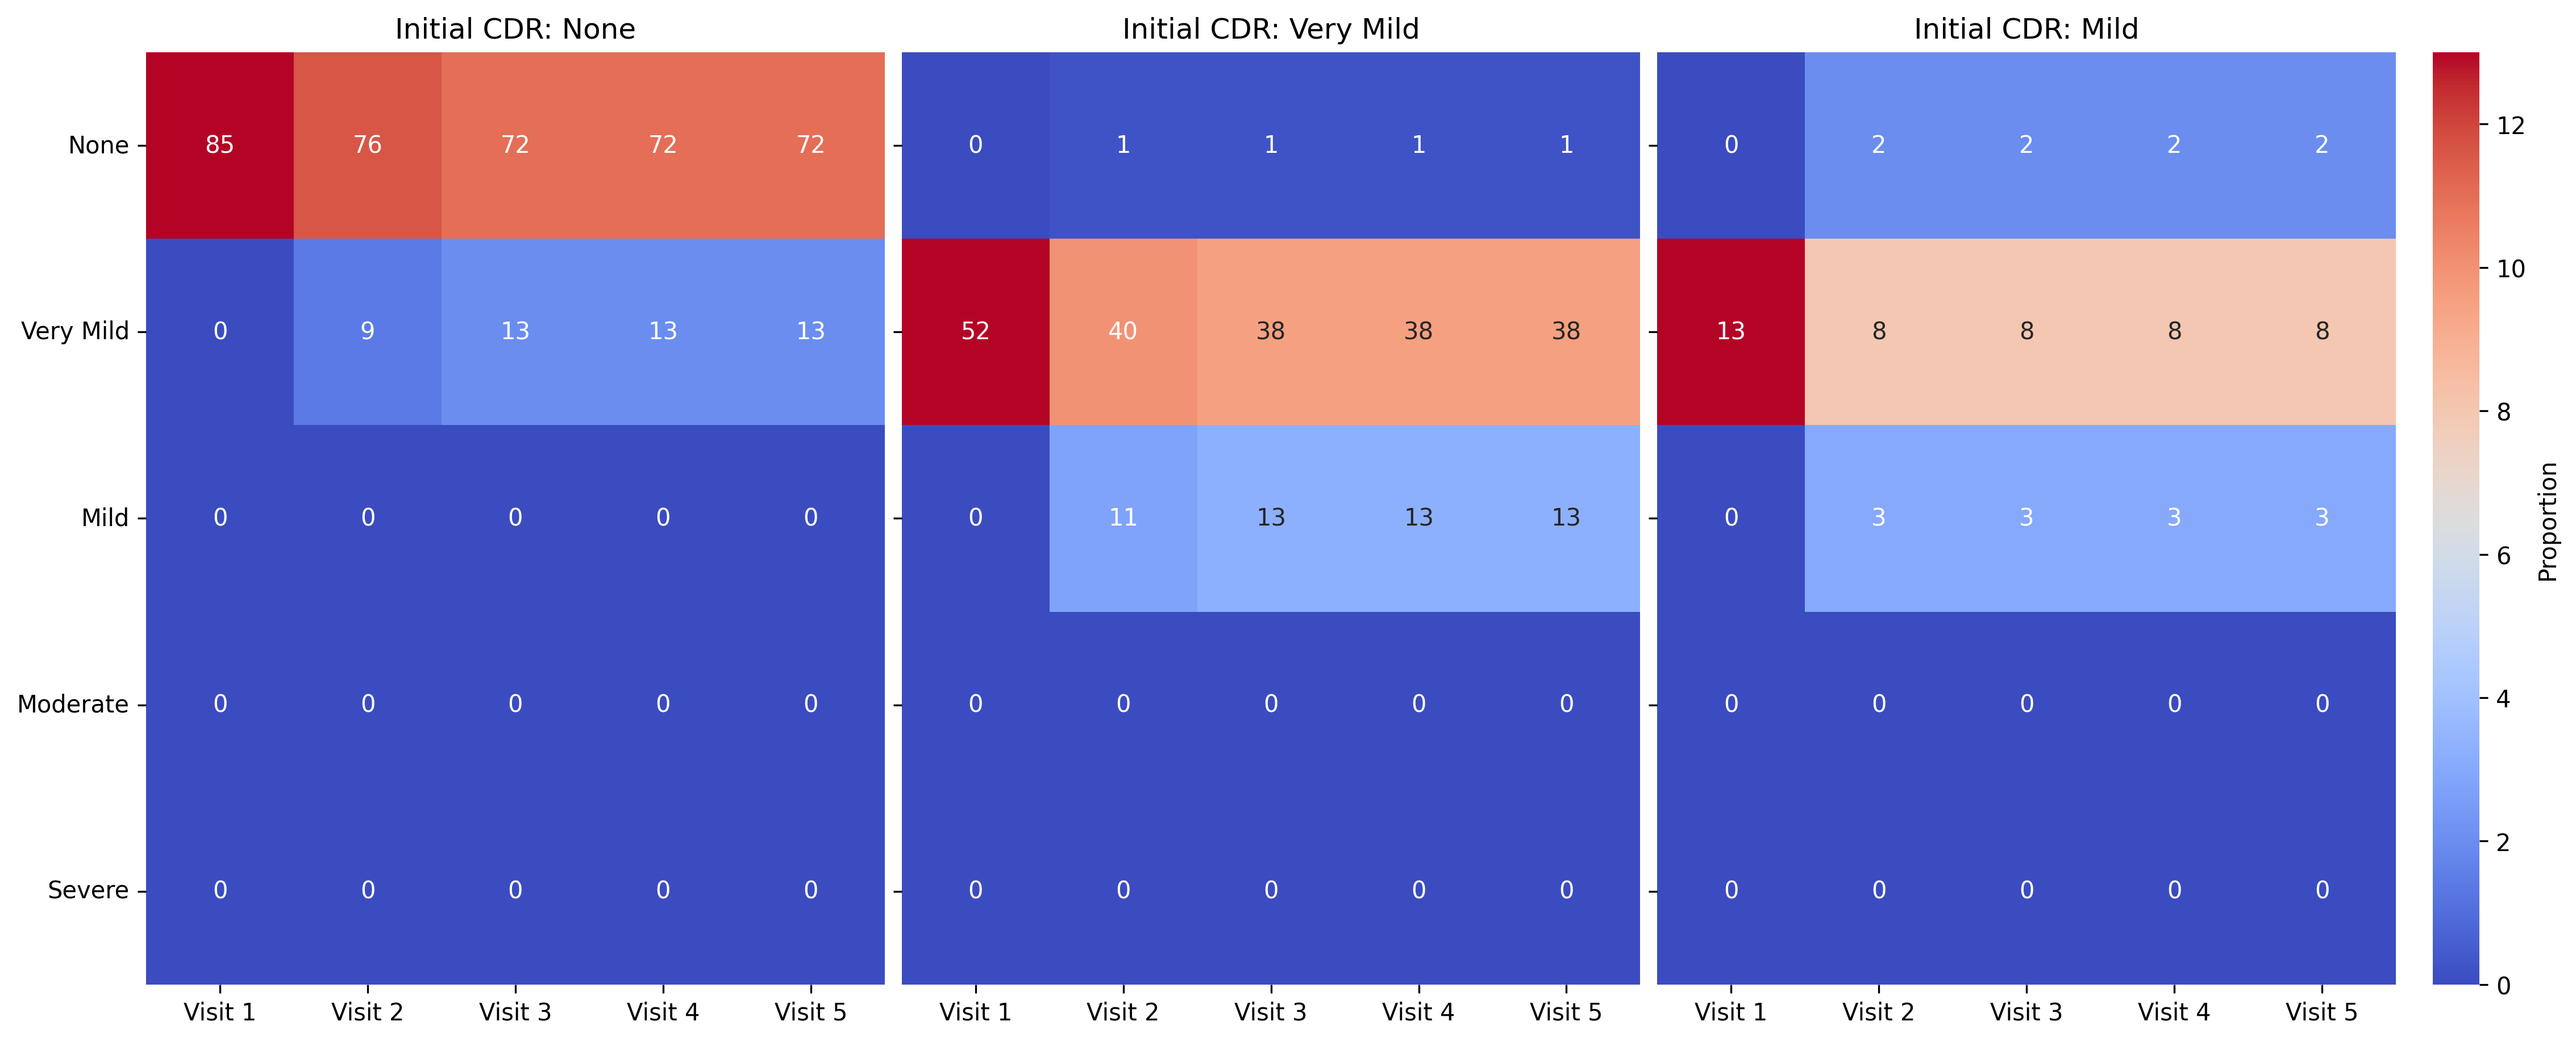
\includegraphics[width=400px]{2_disease_progression_over_time.png}
  \caption{Disease progression over time grouped by started level condition.}
  \label{fig:disease-progression-2}
\end{figure}


Different regularization penalties were tested, with results in Table \ref{tab:penalties-results-2}. The model without regularization achieved the highest mean ROC-AUC, slightly better than other penalties, followed by the L2 penalty. However, both scores are only marginally better than random guessing, indicating limited predictive power. The L1 penalty resulted in a mean ROC-AUC below random guessing, showing its ineffectiveness. These results highlight the need for careful regularization selection to optimize performance. Despite slightly better results with no regularization and the L2 penalty, overall performance is inadequate for clinical use risking misdiagnosis. Improving model performance and reliability is crucial before clinical deployment, requiring addressing data imbalance, enhancing training, and validating with comprehensive datasets.


\begin{table}[h]
\centering
\begin{tabular}{ccccc}
\toprule
Penalty & Mean ROC-AUC & ROC-AUC 95\% CI & Mean F1 & F1 95\% CI \\
\midrule
NO & 0.554 & [0.544 , 0.564] & 0.225 & [0.128 , 0.323] \\
L1 & 0.484 & [0.481 , 0.488] & 0.182 & [0.173 , 0.192] \\
L2 & 0.552 & [0.549 , 0.555] & 0.210 & [0.19 , 0.23] \\
\bottomrule
\end{tabular}
\caption{

    Training scores for each regularization configuration.
}
\label{tab:penalties-results-2}
\end{table}



\pagebreak
\section{Task 3 - advanced ML}
\subsection{Methods}

\begin{enumerate}
\item Load the appointments and participants datasets. Perform a left join of participants into appointments, ensuring correct data types. Exclude patients with fewer than 5 appointments and remove the participant ID column, as IDs are irrelevant for model decisions.
\item Develop a pipeline for the column transformer (see Figure \ref{fig:pipeline-3}). Incorporate imputers, scalers, and encoders. Use a one-hot encoder for non-ordinal categories and handle unknown values to accommodate dataset variations.
\item Select algorithms to test: Support Vector Machine (SVM), Random Forest (RF), and Gradient Boosting (GB). Define parameter grids for each:
 \begin{itemize}
    \item SVM grid: kernel (linear, rbf), C (0.1, 0.5, 0.7, 1), class-weight (balanced), gamma (scale, auto).
    \item RF grid: n\_estimators (300, 400), max\_depth (None, 10), min\_samples\_leaf (1, 3), bootstrap (True), criterion (gini), class-weight (balanced).
    \item GB grid: learning rate (0.1, 0.5), n\_estimators (300, 400), max\_depth (3, 5).
    \end{itemize}
\item For each algorithm, construct a pipeline with the column transformer, feature selector, and grid search as the classifier (see Figure \ref{fig:pipeline-3}). Use nested cross-validation with 6 outer and 2 inner shuffled folds. Select the best algorithm based on the F1 score, which effectively measures positive class prediction (no-show).
\item Generate precision-recall curves and aggregate predictions from the best models to create a pooled confusion matrix for each outer fold. Use permutation importance to assess feature impact on positive class predictions with the best model.
\item Implement a Stacking Classifier with Logistic Regression as the final estimator. Stack the best models from all tested algorithms in the initial grid search, excluding the top-performing algorithm. Use the same pipeline setup as the best algorithm but replace the grid with the stacking classifier (see Figure \ref{fig:pipeline-3}).
\item Plot learning curves for both the top-performing algorithm and the stacking classifier.
\end{enumerate}



\begin{figure}[h]
  \centering
  \includegraphics[width=400px]{task3.png}
  \caption{Set pipeline as a flow diagram.}
  \label{fig:pipeline-3}
\end{figure}
% need to make a flow to show the process
\subsection{Results}

To find the best algorithm and hyperparameters for predicting missed appointments, various combinations were analyzed. Random Forest (RF) proved most effective, using these hyperparameters:
\begin{itemize}
\item Bootstrap: True;
\item Class weight: balanced;
\item Criterion: gini;
\item Max Depth: 10;
\item Min Samples per Leaf: 3;
\item Estimators: 400;
\end{itemize}

RF outperformed Support Vector Machine (SVM) and Gradient Boosting (GB) in ROC-AUC and F1 scores (Table \ref{tab:algorithms-performances-3}). The F1 score shows moderate prediction ability, while this score indicates that the model is the best among the tested options, it also indicates a margin for improvement.

\begin{table}[h]
\centering
\begin{tabular}{lrr}
\toprule
Algorithm & ROC AUC & F1 \\
\midrule
SVC & 0.662 & 0.394 \\
RF & 0.734 & 0.452 \\
GB & 0.7182 & 0.406 \\
\bottomrule
\end{tabular}
\caption{
    Classifier algorithms performance (in the same pipeline).
}
\label{tab:algorithms-performances-3}
\end{table}

\begin{figure}[h]
  \centering
  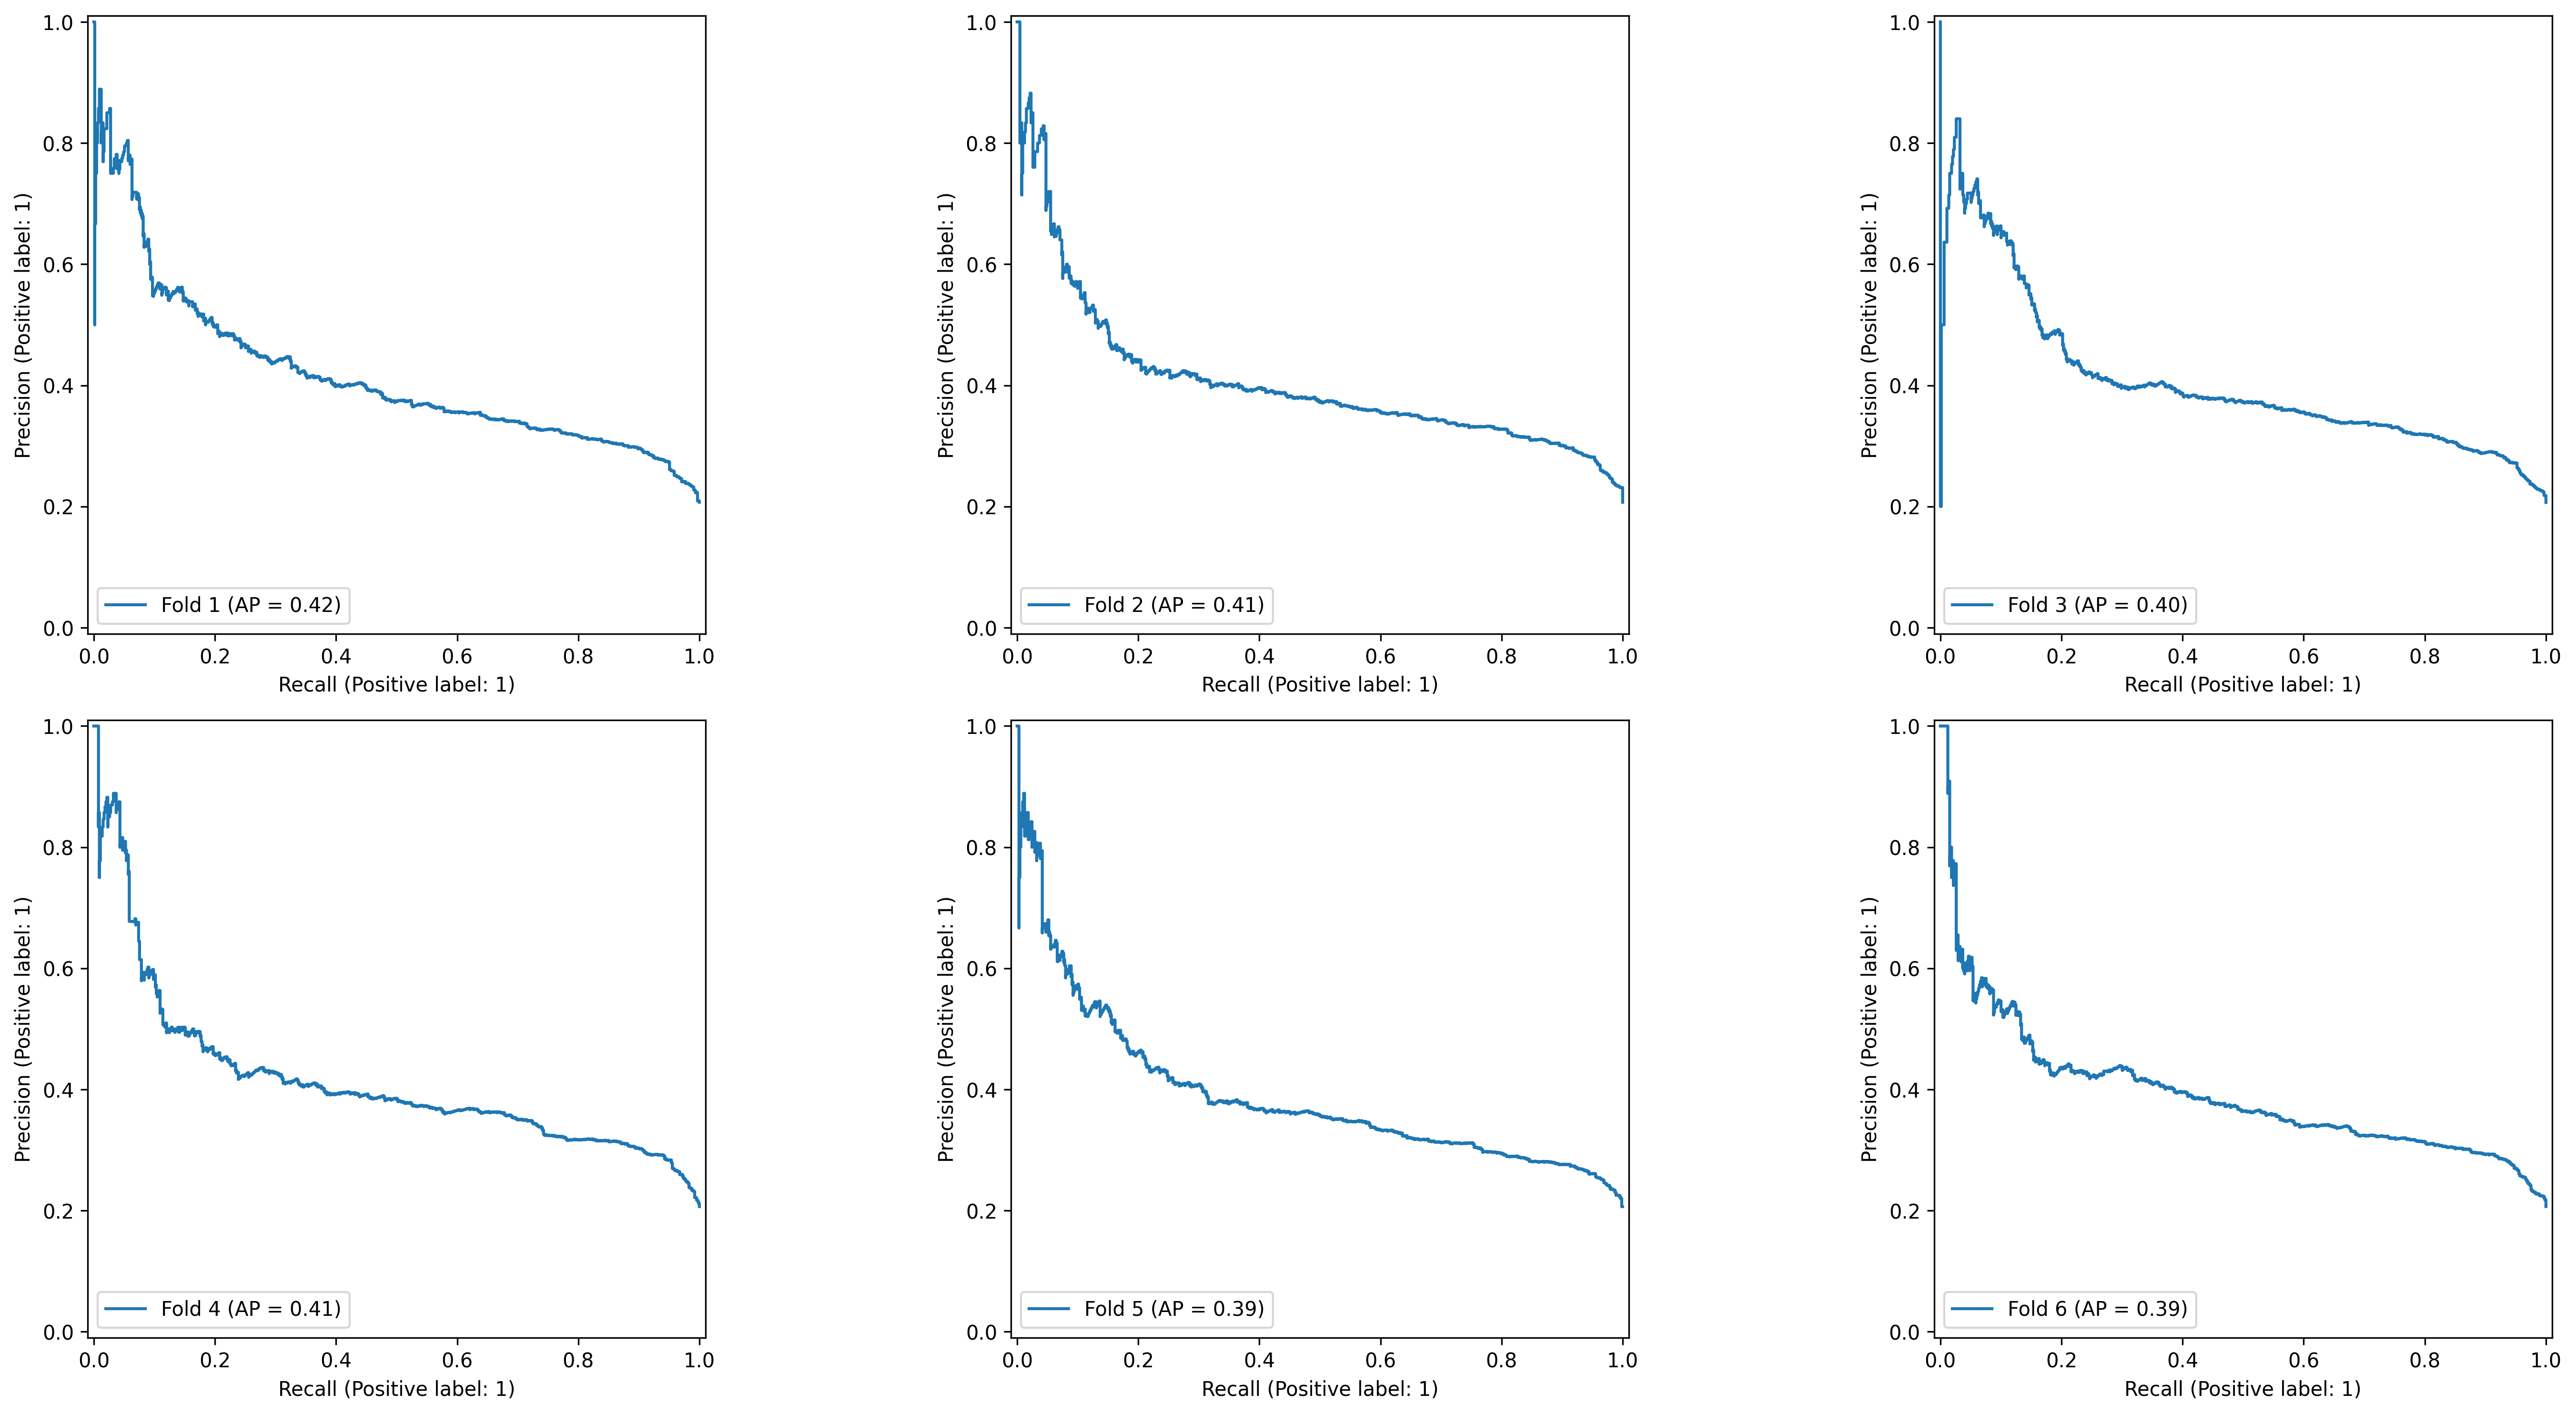
\includegraphics[width=400px]{3_precision_recall_curve_folds.png}
  \caption{Single classifier precision-recall curves for each fold.}
  \label{fig:precision-recall-curves-3}
\end{figure}

Key features include scheduling time, age, total visits, appointment date, and SMS reminders (Figure \ref{fig:feature-importances-3}). These key features are indispensable for users to provide to the model, as they are the most impactful on predicting the no-show class, enabling insightful predictions and help in targeted interventions like extra reminders for patients. The precision-recall curve (Figure \ref{fig:precision-recall-curves-3}) shows high precision but low recall for every cross validation fold, missing many positives, likely due to class imbalance or feature issues. The pooled confusion matrix (Figure \ref{fig:pooled-confusion-matrix-3}) that mimics the behaviour for the whole model using each fold, shows 2,000 missed no-shows and 3,000 false positives, with 1,600 correct no-show predictions, further illustrating the challenge of correctly predicting that class.



\begin{figure}[h]
  \centering
  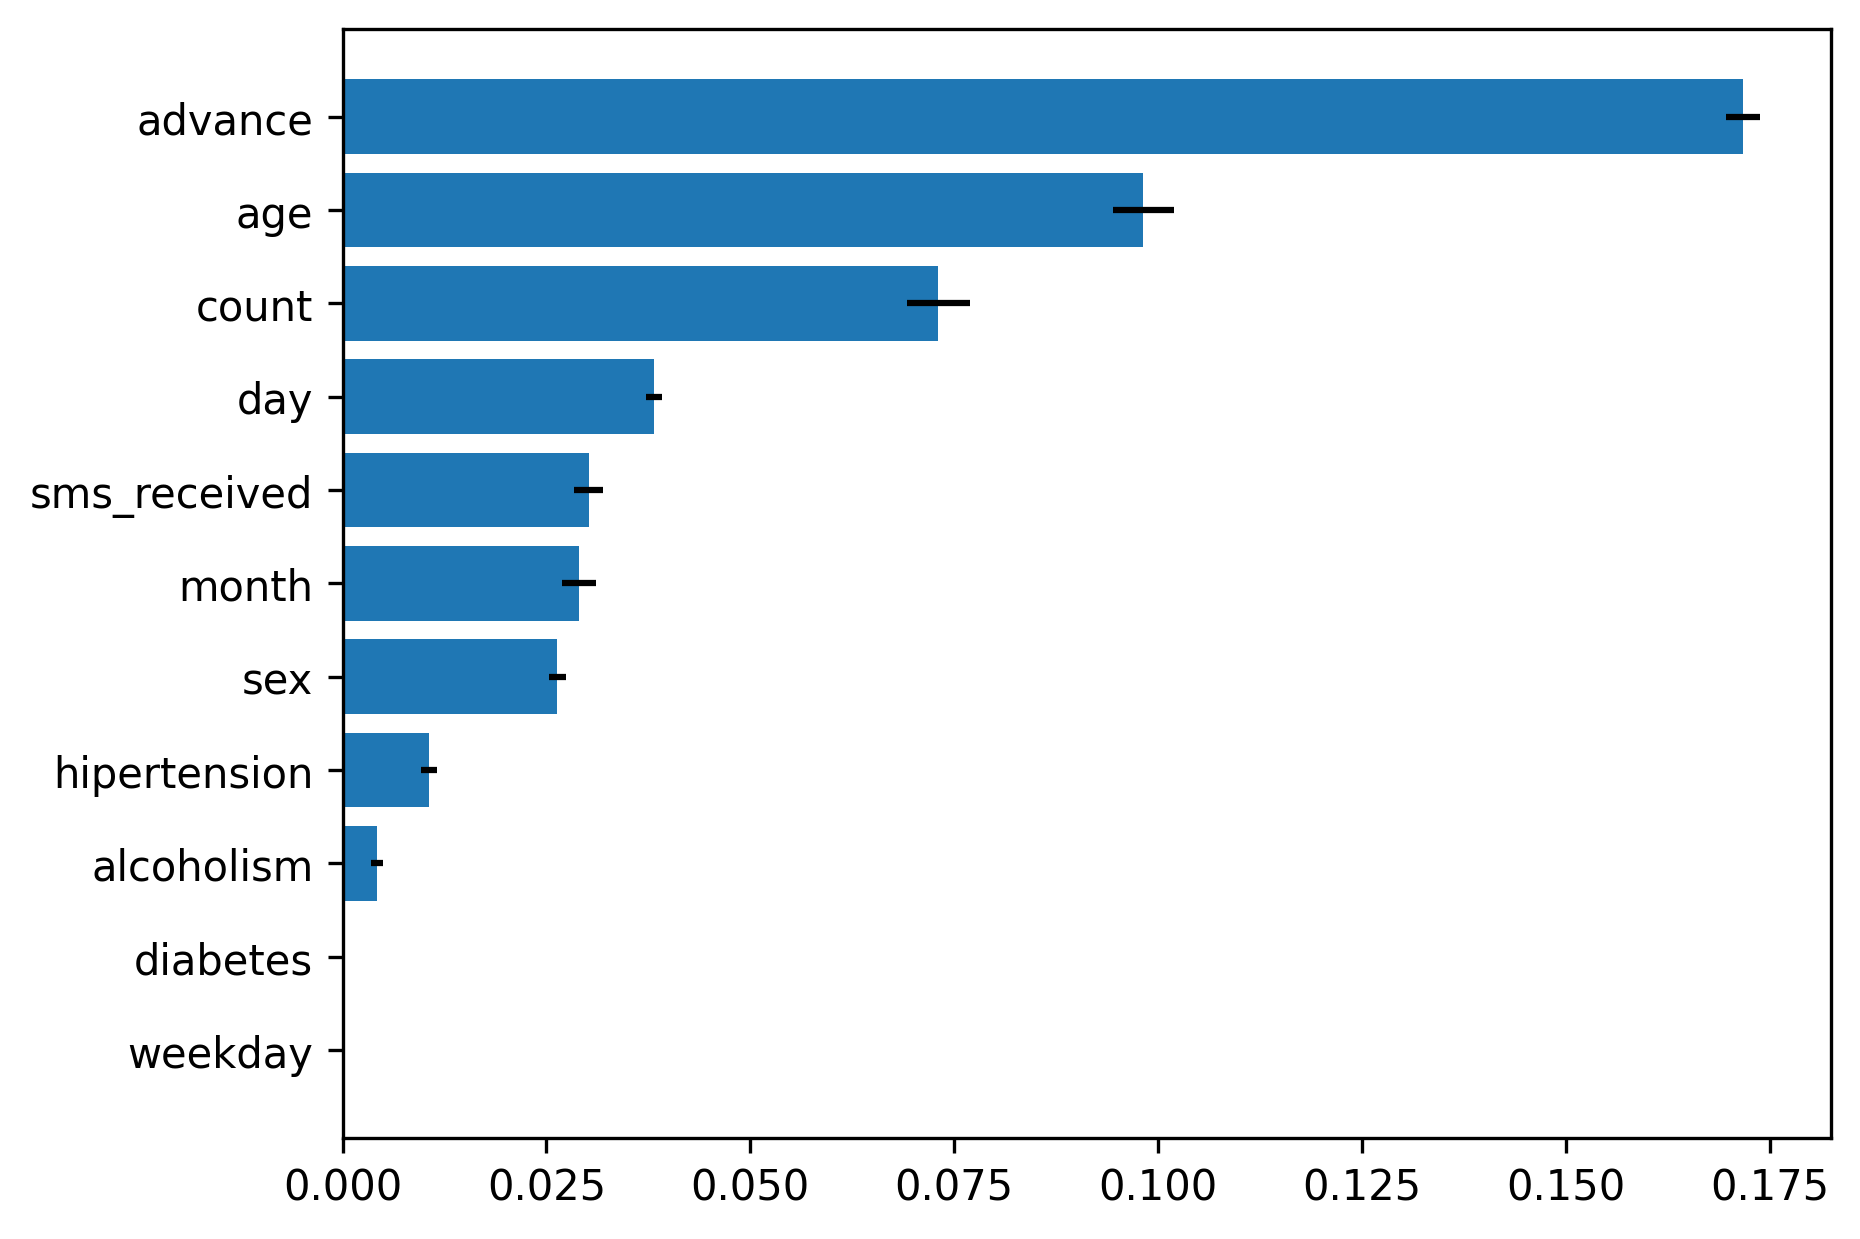
\includegraphics[width=300px]{3_feature_importances_permutation.png}
  \caption{Features impact on the best model output (no-show class).}
  \label{fig:feature-importances-3}
\end{figure}

A stacking model was considered to improve the prediction ability of the model, but RF excelled in the validation scores, which is more important to determine the generalization capability of a model. The learning curve (Figure \ref{fig:learning-curves-3}) shows RF's validation score improves with more data, reducing noise. The stacking model's learning curve showed faster validation improvement but was less robust than RF for this task when the data samples were all covered.


\begin{figure}[h]
  \centering
  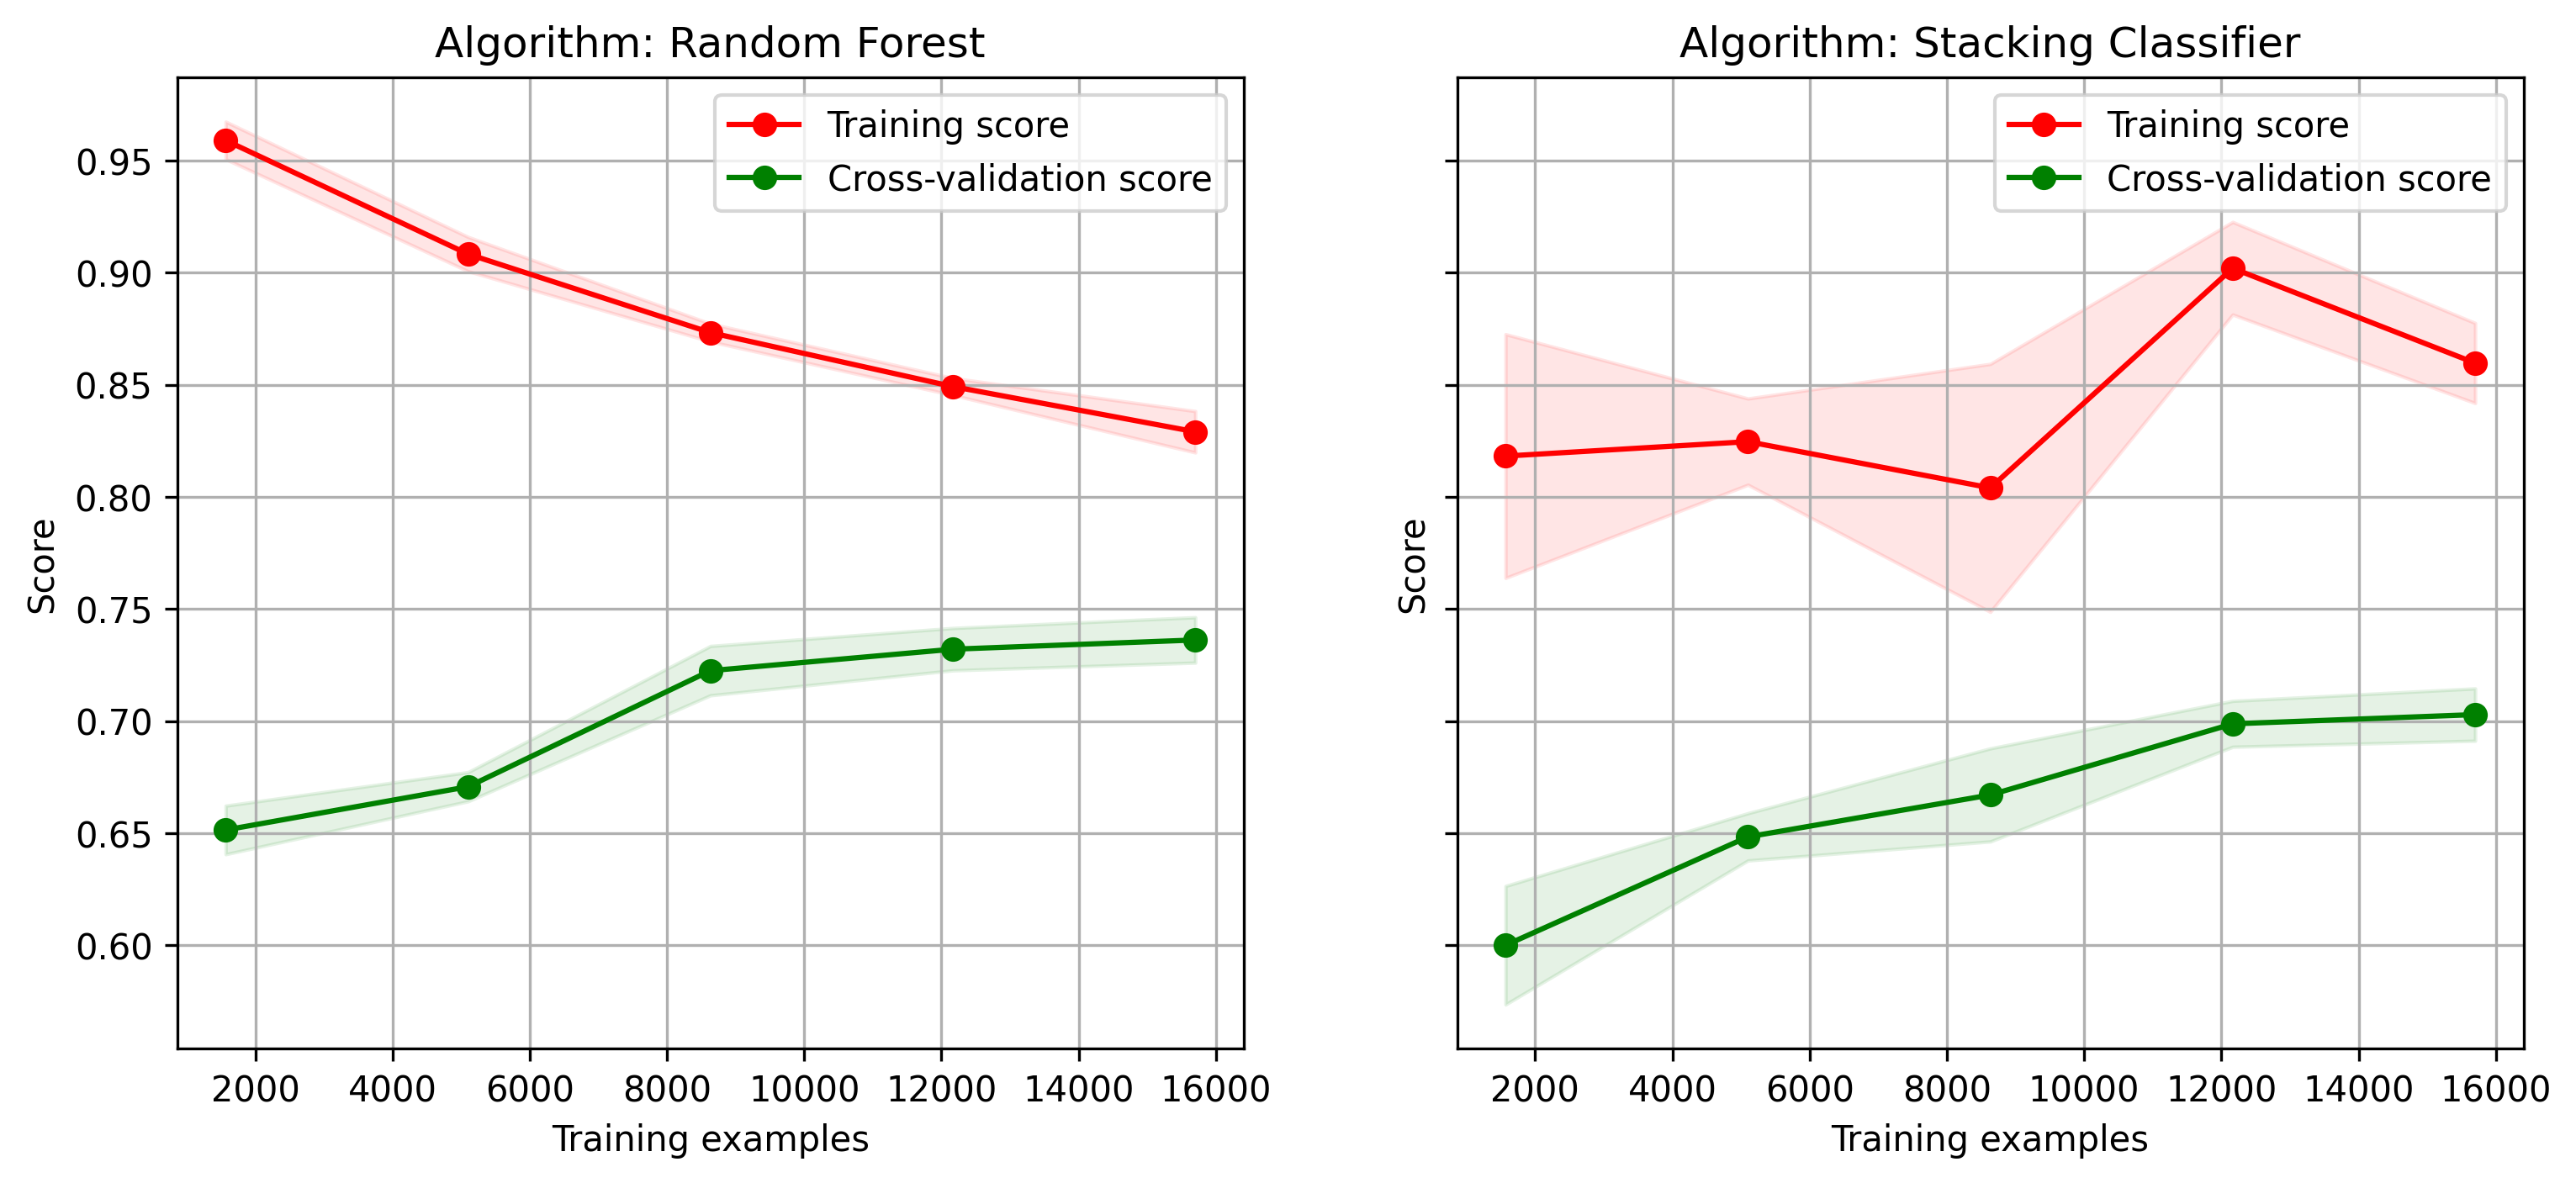
\includegraphics[width=400px]{3_learning_curves.png}
  \caption{Single and stacked classifiers learning curves.}
  \label{fig:learning-curves-3}
\end{figure}

In summary, the RF algorithm, with tuned hyperparameters, is the best choice for predicting appointment no-shows, despite needing improved recall. Its robustness makes it valuable for healthcare providers, offering insights to reduce no-shows and conserve resources. By leveraging key features, it aids in deciding on patient reminders, though not for diagnosis. With no significant negative consequences, it is suitable for deployment, and its performance can improve with more no-show data. The current baseline provides a solid foundation for future enhancements.


\begin{figure}[h]
  \centering
  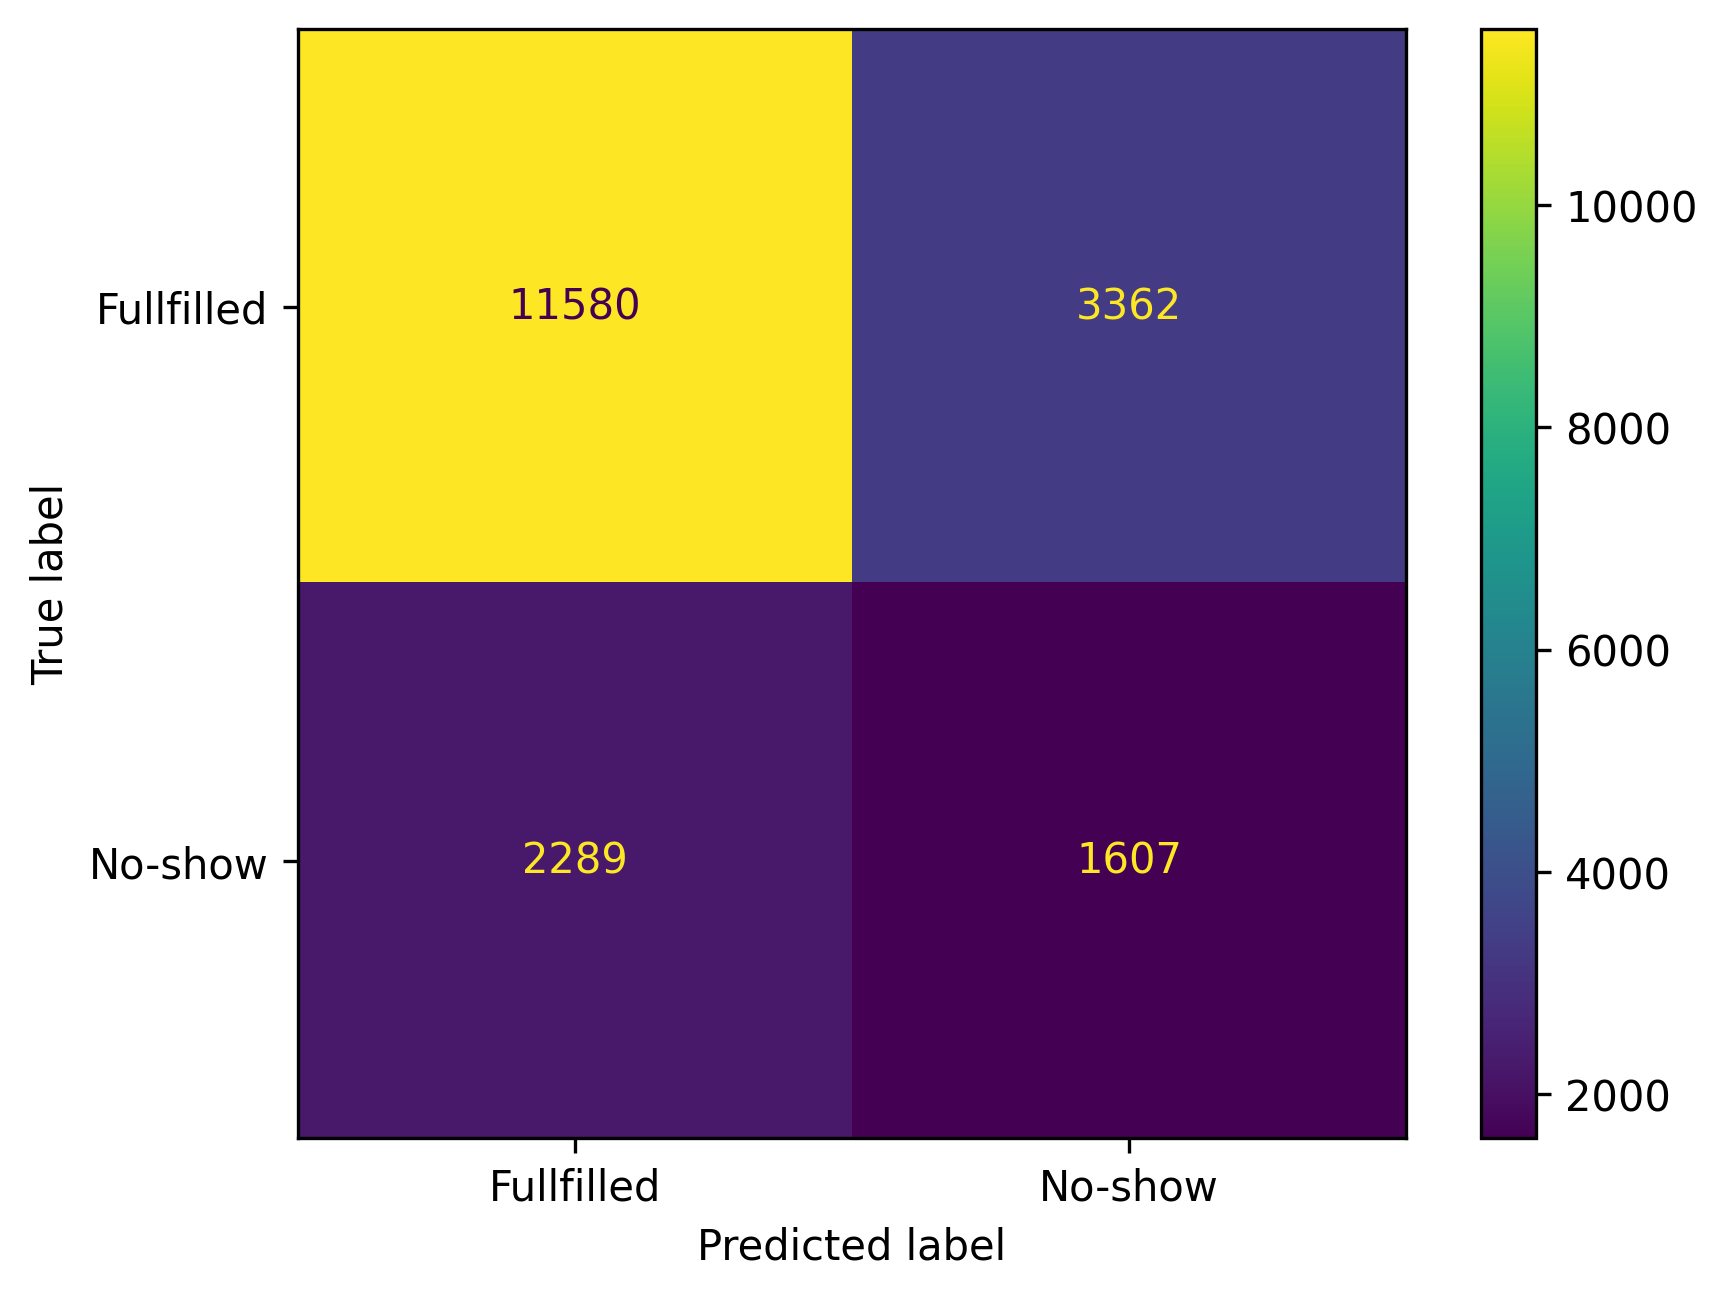
\includegraphics[width=300px]{3_combined_confusion_matrices.png}
  \caption{Single model pooled confusion matrix.}
  \label{fig:pooled-confusion-matrix-3}
\end{figure}


\pagebreak
\section{Task 4 - deep learning}
\subsection{Methods}
\begin{enumerate}
    \item Gather domain names, superfamily names, and CATH IDs for each sequence. Join this data into one dataset, using CATH ID and domain name as keys. Exclude sequences in superfamilies with fewer than 1000 occurrences and those without a superfamily name. Retain only the sequences and superfamily names columns in the final dataset.
    \item Convert labels to binary; transform sequences into vectors; pad sequences to a max length of 300 (Figure \ref{fig:pipeline-4}).
    \item Use a random search tuner to build a transformer, optimizing validation loss over 10 trials. Decide on embedding dimensions (16 or 32), encoder layers (2 or 4), heads per layer (2 or 4), dense layers (1 or 2), units per layer (32 or 64), and learning rate (0.001 or 0.01) for the Adam optimizer. Use accuracy and AUC as metrics. Transformer architecture is in Figure \ref{fig:pipeline-4}.
    \item Implement a 4-fold splitter for cross-validation, separating test and train datasets for evaluation and hyperparameter tuning.
    \item For each fold, train the model for 50 epochs using the best hyperparameters. Record train, validation, and evaluation performance, and the top 5 tuner trials to assess hyperparameter impact.
    \item Identify the best epoch by lowest validation loss. Repeat the previous step with optimized epochs.
    \item Calculate fold means for cross-validation; plot performance graphs for chosen epochs and display tables with trial and fold results for analysis.
\end{enumerate}

\begin{figure}[h]
  \centering
  \includegraphics[width=400px]{task4.png}
  \caption{Preprocessing and transformer architecutre.}
  \label{fig:pipeline-4}
\end{figure}



\subsection{Results}


% How well can we predict the protein function (CATH superfamily) from its sequence?

Predicting protein function (CATH superfamily) from sequences using a neural network shows promise. The model uses a transformer architecture with encoder components to leverage attention mechanisms, focusing on each protein sequence letter to identify crucial patterns. This makes transformers ideal for sequence processing.

Performance was tested with various encoder layers, attention heads, dense layers, and learning rates (Table \ref{tab:losses-hyperparameters-4}). Results show smaller learning rates improve loss, suggesting they allow more effective learning with more epochs. More attention heads and a single dense layer performed best with a higher learning rate.


\begin{table}[h]
\centering
\begin{tabular}{r|rrrrr}
\toprule
Loss & Encoder Layers & Heads/encoder & Dense Layers & Units/dense layer & Learning Rate\\
\midrule
2.378  & 2 & 2-4 & 1 & 32 & 0.001\\
2.847  & 2 & 4-4 & 2 & 32-32 & 0.01\\
2.996  & 2 & 2-4 & 1 & 64 & 0.01 \\
3.094  & 2 & 2-2 & 2 & 64-64 & 0.01 \\
3.299  & 4 & 2-2-4-2 & 1 & 64-32  & 0.01\\
\bottomrule
\end{tabular}
\caption{
    Different losses results from different hyperparameters combinations.
}
\label{tab:losses-hyperparameters-4}
\end{table}

\begin{table}[h]
\centering
\begin{tabular}{lrrr}
\toprule
Fold & Loss & Accuracy & AUC \\
\midrule
 1 & 2.549 & 0.478 & 0.917 \\
 2 & 2.493 & 0.475 & 0.925 \\
 3 & 2.471 & 0.489 & 0.926 \\
 4 & 2.433 & 0.475 & 0.928 \\
\cmidrule{1-4}
Mean & 2.487 & 0.479 & 0.924 \\
\bottomrule
\end{tabular}
\caption{
    Cross validation results.
}
\label{tab:cross-validation-4}
\end{table}

Four-fold cross-validation with a separate test set was used to avoid data leakage during hyperparameter tuning. Overfitting was observed at 50 epochs, where training loss decreased but validation loss increased after a point (Figure \ref{fig:50-epochs-4}). The optimal epoch count was found by minimizing validation loss, and the model was retrained (Figure \ref{fig:best-epoch-4}), enhancing generalization. The model's mean AUC was 0.920 (Table \ref{tab:cross-validation-4}), showing strong protein function prediction, though accuracy was low, indicating room for improvement in prediction precision.




\begin{figure}[h]
  \centering
  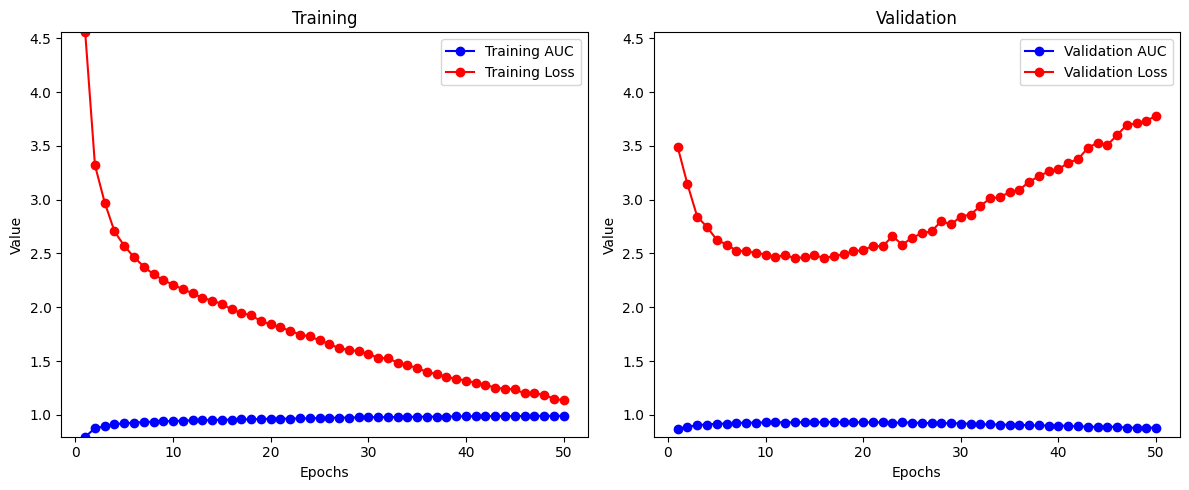
\includegraphics[width=400px]{4_nn_performance_50_epochs.png}
  \caption{Model performance with 50 epochs training.}
  \label{fig:50-epochs-4}
\end{figure}

\begin{figure}[h]
  \centering
  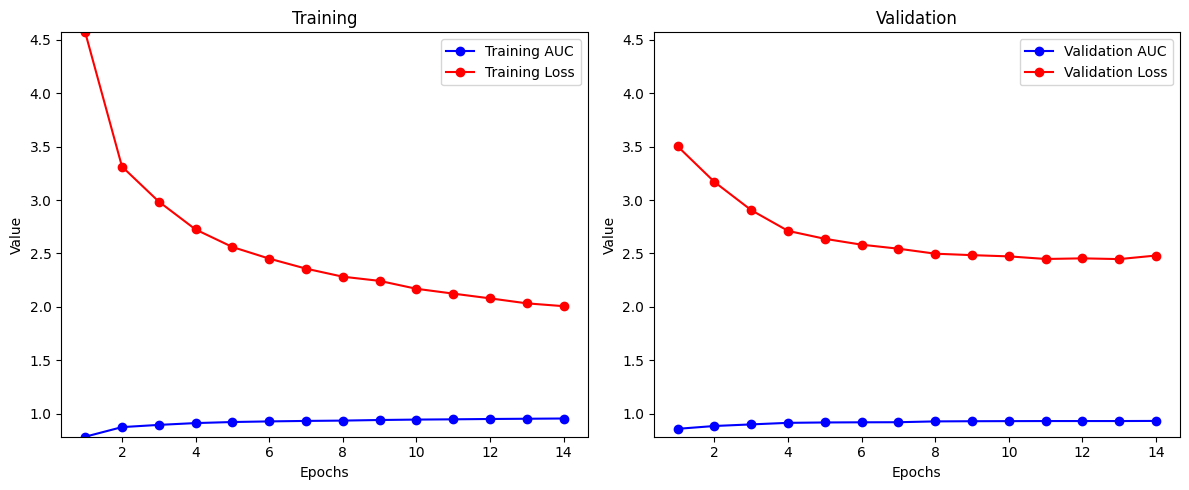
\includegraphics[width=400px]{4_nn_performance_best_epoch.png}
  \caption{Optimized model performance with the best amount of epochs.}
  \label{fig:best-epoch-4}
\end{figure}




The dataset's characteristics influenced model performance. The S60 dataset, with more occurrences per protein family, helped the model capture sequence patterns better than the non-redundant S40 dataset. This richer data improved the model's ability to predict protein functions, achieving an AUC near 95\%, showing promise for medical applications like disease understanding and therapy development. However, despite its strong predictive capabilities, the model isn't infallible. Experimental validation and further analyses are necessary to ensure accuracy and reliability in medical contexts.







\pagebreak
\section{Task 5 - image classification}
\subsection{Methods}
\begin{enumerate}
    \item Load the train, validation, and test sets, storing labels and images separately. Load images in two formats: as grayscale with a resolution of 128x128 for the single model (grayscale is chosen because retinal OCT images are typically grayscale, and converting them reduces noise, aiding pattern recognition), and as RGB with a resolution of 224x224 for the transfer model (required for the transfer model's input layer). Compute class weights to ensure balanced tuning and training. Normalize images to a [0,1] range by dividing each pixel by 255 and convert classes to binary class matrices.
    \item Develop the CNN model as illustrated in Figure \ref{}. Use an Adam optimizer with a tuned learning rate (options: 0.001 and 0.01). Set accuracy and AUC as metrics. Implement a random search tuner aimed at maximizing validation AUC, with a maximum of 10 trials.
    \item After hyperparameter tuning with the specified tuner and a batch size of 128, train the CNN for 36 epochs using the same batch size and the computed class weights. Save the top 3 trials and evaluate the network with the test subsets.
    \item Construct the transfer model as depicted in Figure \ref{}, utilizing the VGG16 pre-trained model without its top layer, and set its weight to not trainable, to leverage proper feature extraction. Use an Adam optimizer with a learning rate of 0.000001. Employ the same metrics as the handcrafted network and train the transfer model using the RGB 224x224 subsets for the same number of epochs as before.
    \item For both models, plot the performance metrics for each epoch, generate the confusion matrix for the test subset, and calculate occlusion sensitivity for each class prediction.

\end{enumerate}

\begin{table}[h]
\centering
\begin{tabular}{lrr}
\toprule
Metric & Transfer Model (VGG16) & Simple CNN \\
\midrule
Loss & 0.780 & 0.667 \\
Accuracy & 0.864 & 0.860 \\
AUC & 0.969 & 0.959 \\
\bottomrule
\end{tabular}
\caption{
    Comparison of evaluation metrics between Transfer Model (VGG16) and Simple CNN.
}
\label{tab:comparison-results}
\end{table}

\subsection{Results}
Classifying retinal images to identify eye disorders using deep neural networks yields promising results, particularly when comparing handcrafted Convolutional Neural Networks (CNNs) and transfer learning models. The handcrafted CNN, despite starting with a high initial loss, achieves commendable performance metrics, with an accuracy of 86\% and an AUC of 95.9\%, indicating its capability to classify retinal images effectively (Table \ref{tab:comparison-results}). However, the initial high loss suggests that the model requires more epochs to stabilize and reach optimal performance, as seen in the progression of the training process (Figure \ref{fig:epochs-5}).

\begin{figure}[h]
  \centering
  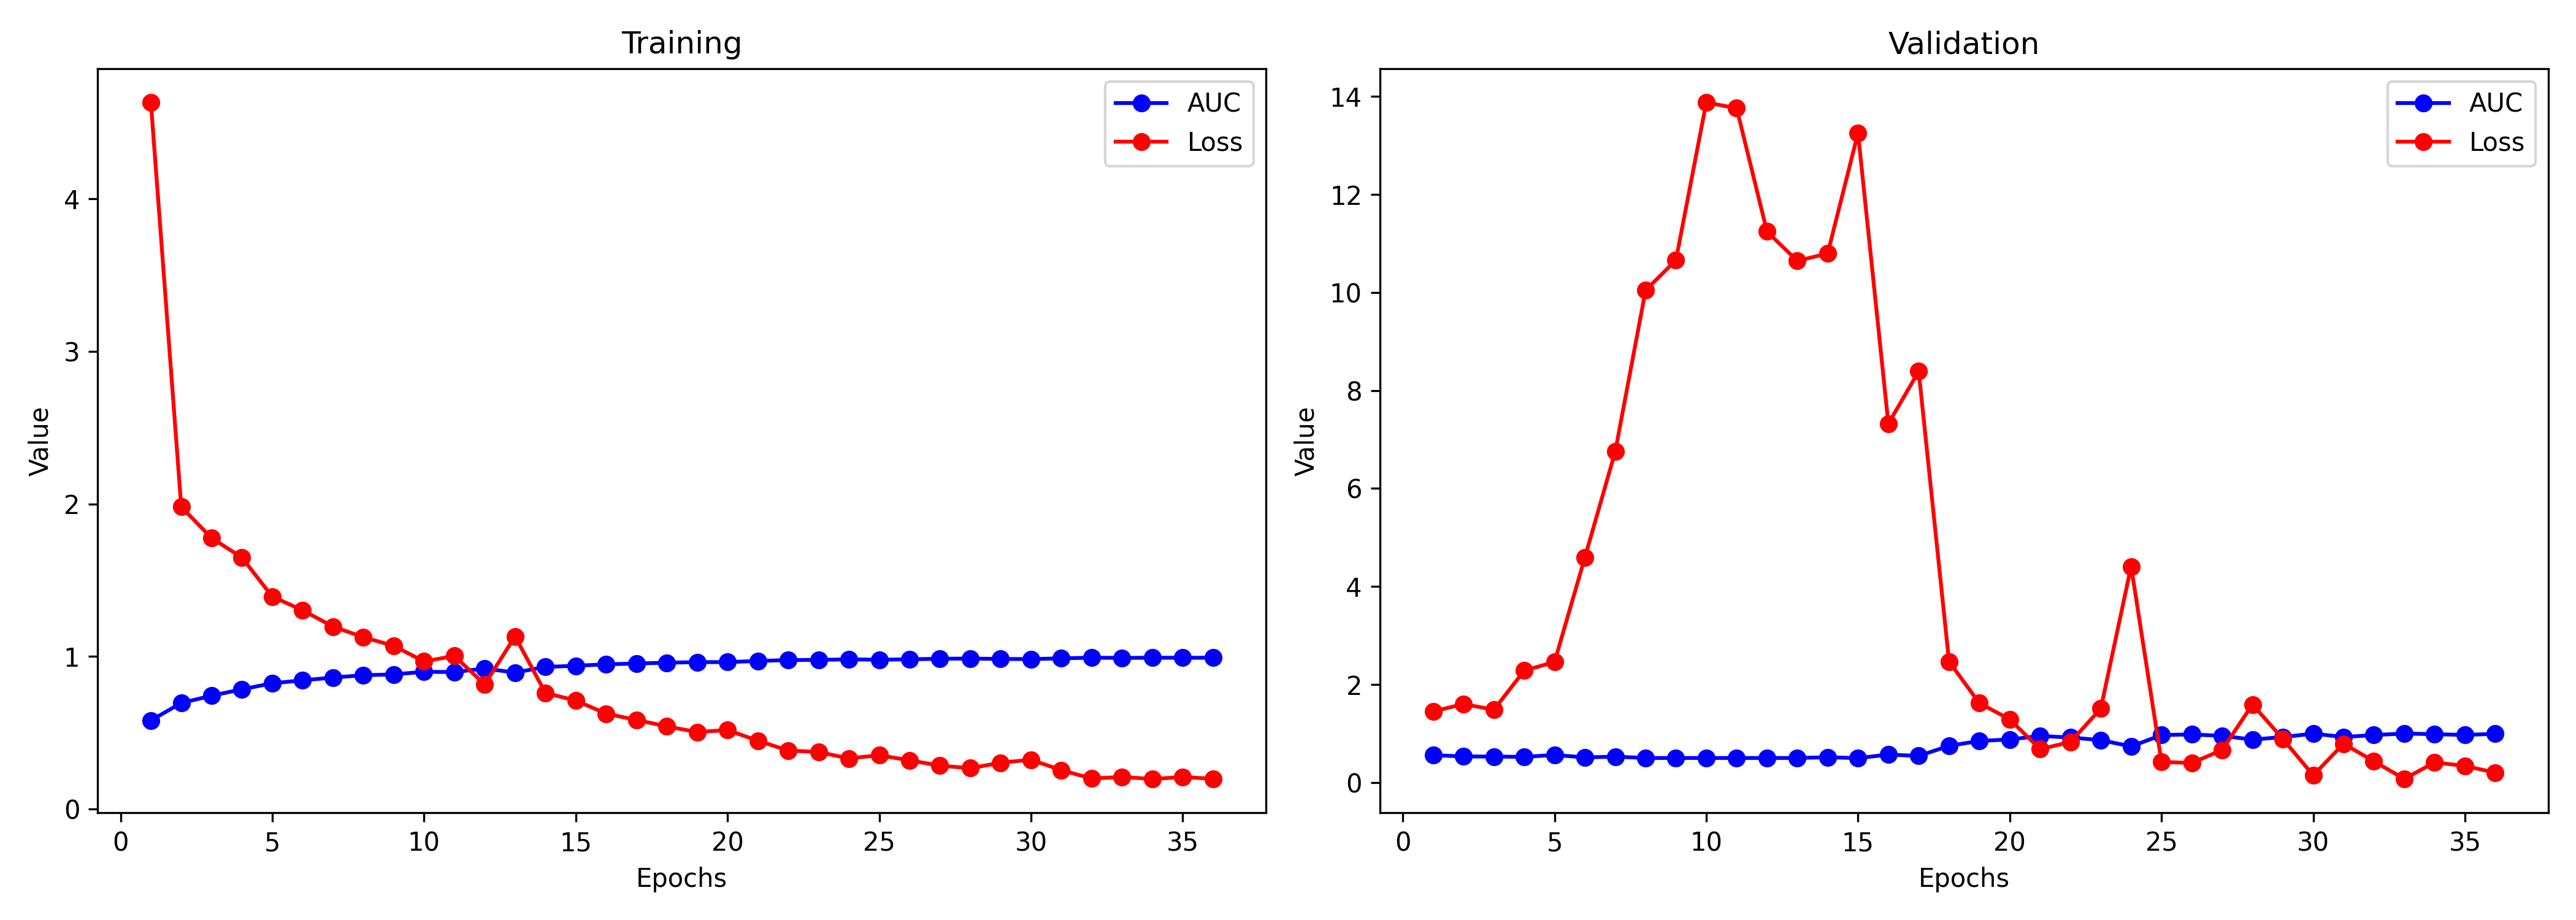
\includegraphics[width=500px]{5_epochs_results.png}
  \caption{Performance of simple CNN for each epoch.}
  \label{fig:epochs-5}
\end{figure}

In contrast, the transfer learning model, built using a pre-trained VGG16 architecture, starts with a significantly lower initial loss (Figure \ref{fig:epochs-transfer-5}), suggesting a more efficient learning process from the outset. The model's ability to maintain a pattern of decreasing loss and increasing AUC over epochs, as seen in the epochs plot (Figure \ref{fig:epochs-transfer-5}), highlights its potential for further improvement and refinement.

\begin{figure}[h]
  \centering
  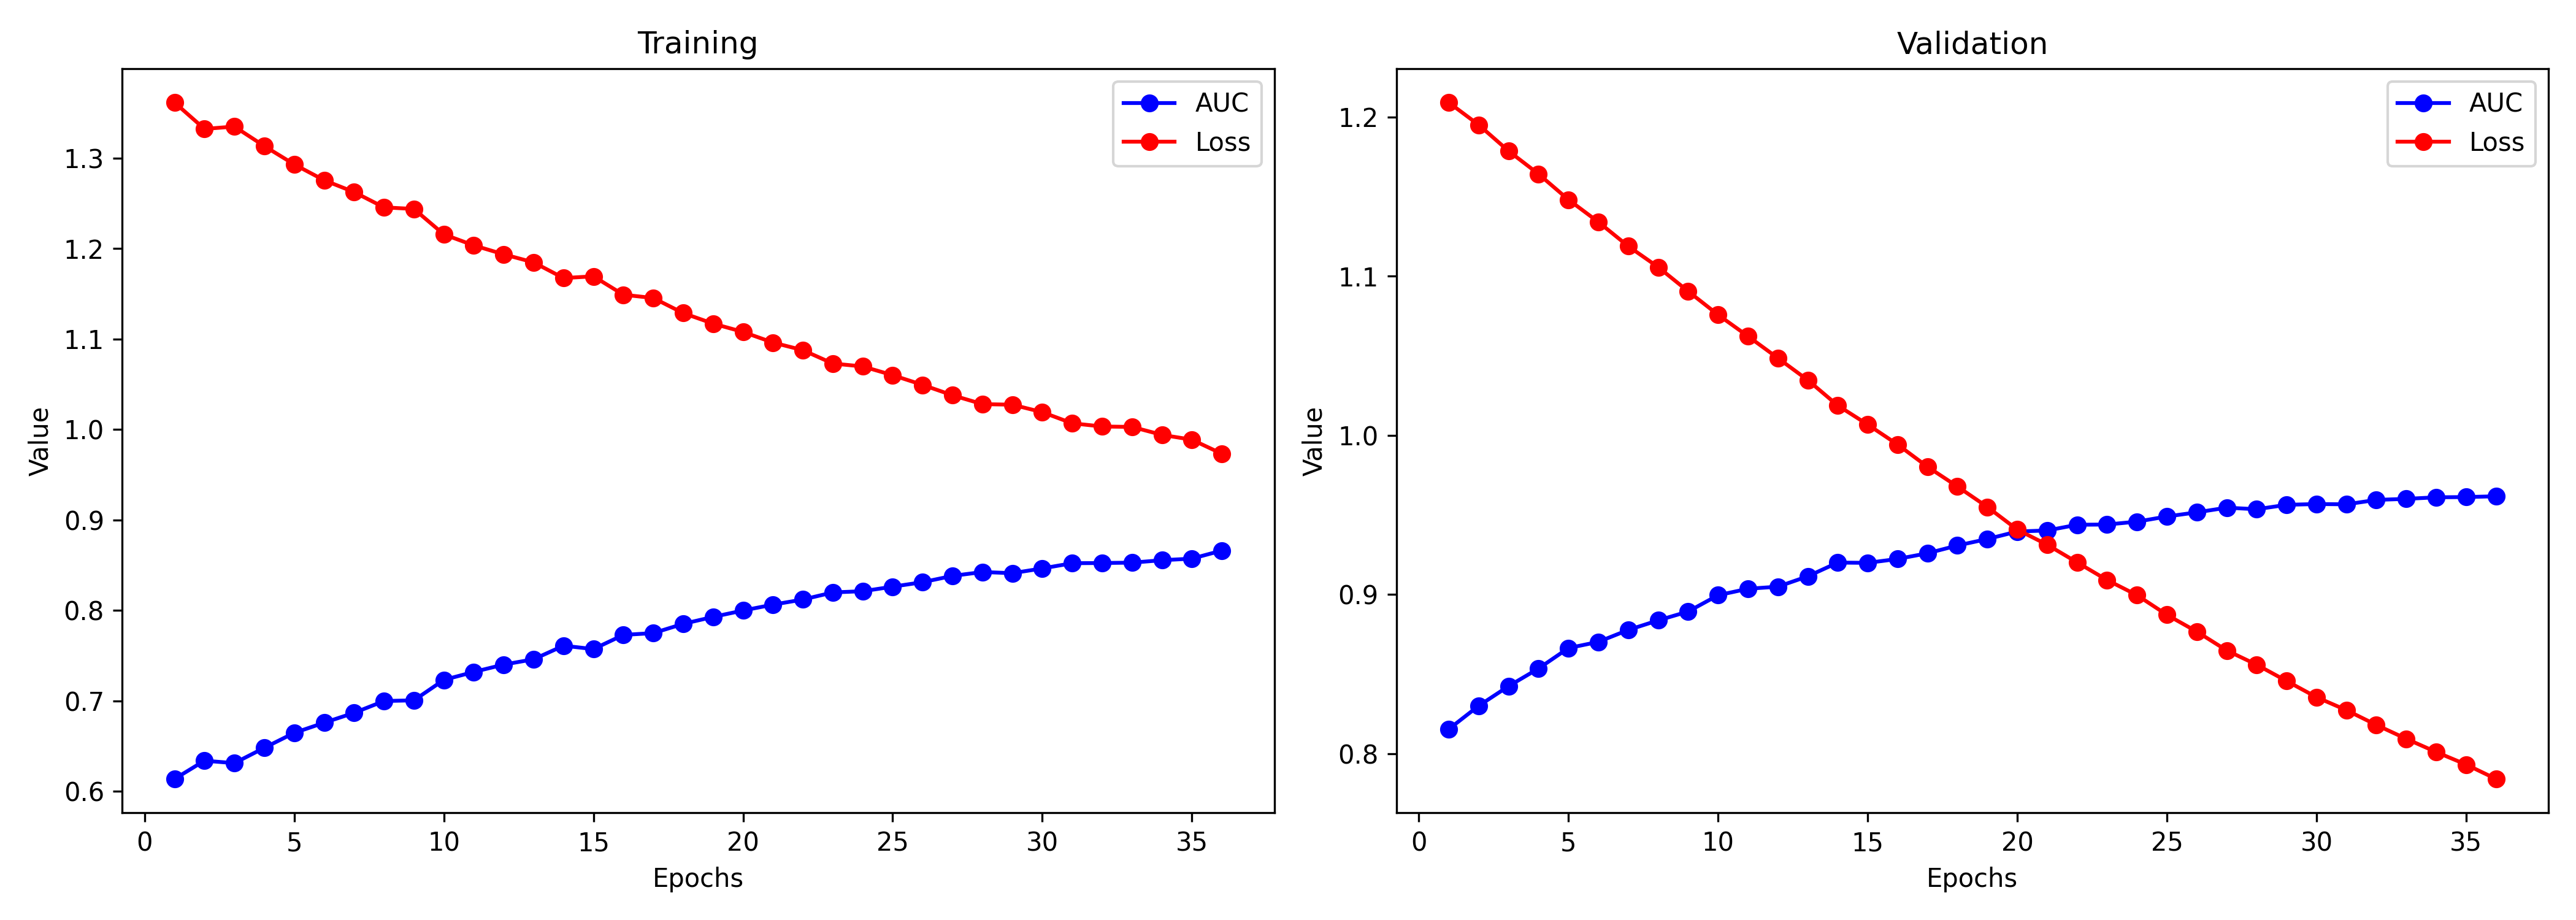
\includegraphics[width=500px]{5_epochs_results_transfer.png}
  \caption{Performance of transfer model for each epoch.}
  \label{fig:epochs-transfer-5}
\end{figure}

The transfer model architecture uses VGG16 as a feature extractor, flattens the output, and feeds it into dense layers with dropout to prevent overfitting, ending with a softmax decision layer. The hand-crafted CNN starts with an input layer, followed by 1-3 convolutional layers (determined by a hyperparameter) with increasing filters, batch normalization, max pooling, and dropout, to avoid overfitting, then flattens the output and passes it through a decision dense layer.


\begin{figure}[h]
  \centering
  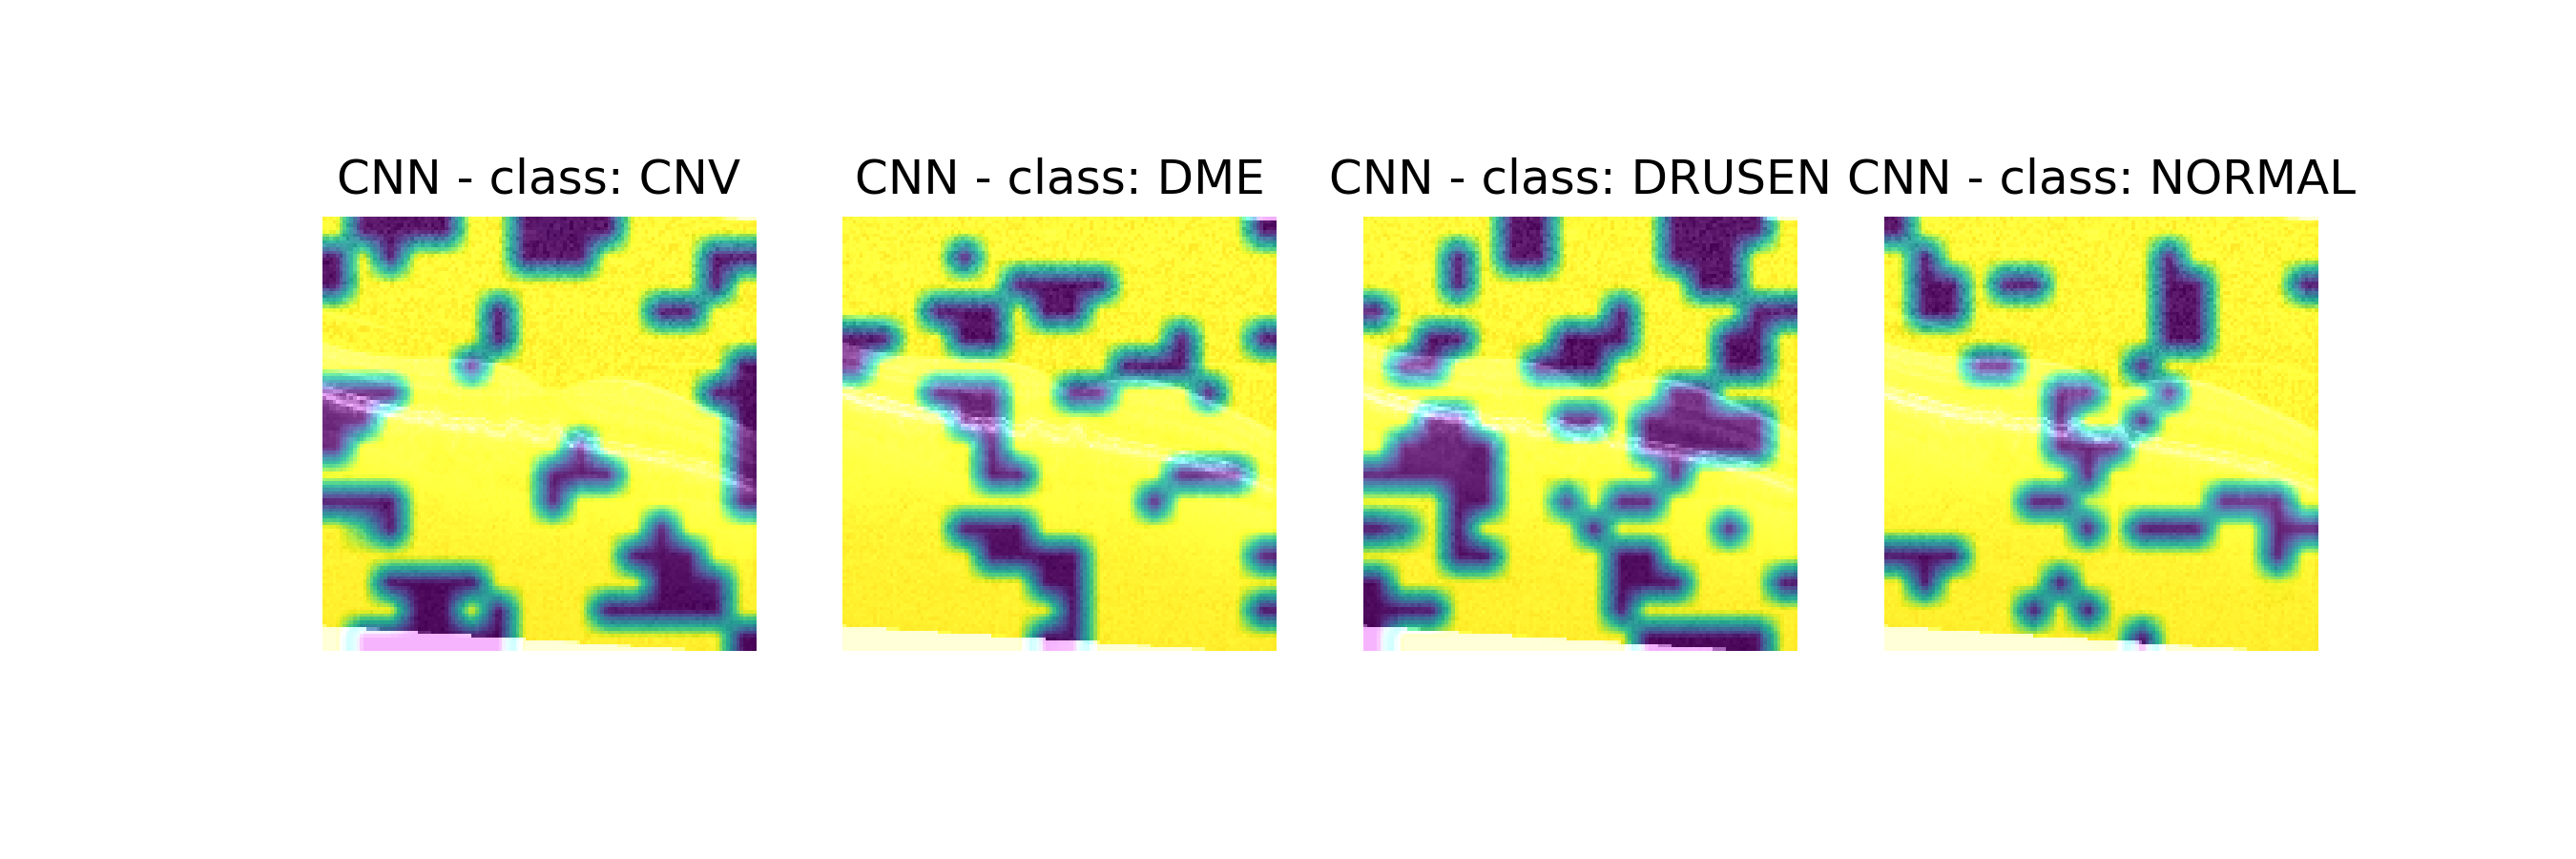
\includegraphics[width=400px]{5_occlusion_sensitivity_cnn.png}
  \caption{Simple CNN occlusion sensitivity per class.}
  \label{fig:occlusion-cnn-5}
\end{figure}

Examining occlusion sensitivity shows that the normal class has fewer focus areas, indicating simpler decision-making, while other classes show more focus areas in both CNN models (Figure \ref{fig:occlusion-cnn-5}). The transfer model has smoother attention areas, suggesting refined feature extraction (Figure \ref{fig:occlusion-transfer-5}), whereas the handcrafted CNN has pixelated attention areas, indicating less sophisticated analysis. The simpler occlusion sensitivity for the normal class is due to its distinct, easily recognizable features.


\begin{figure}[h]
  \centering
  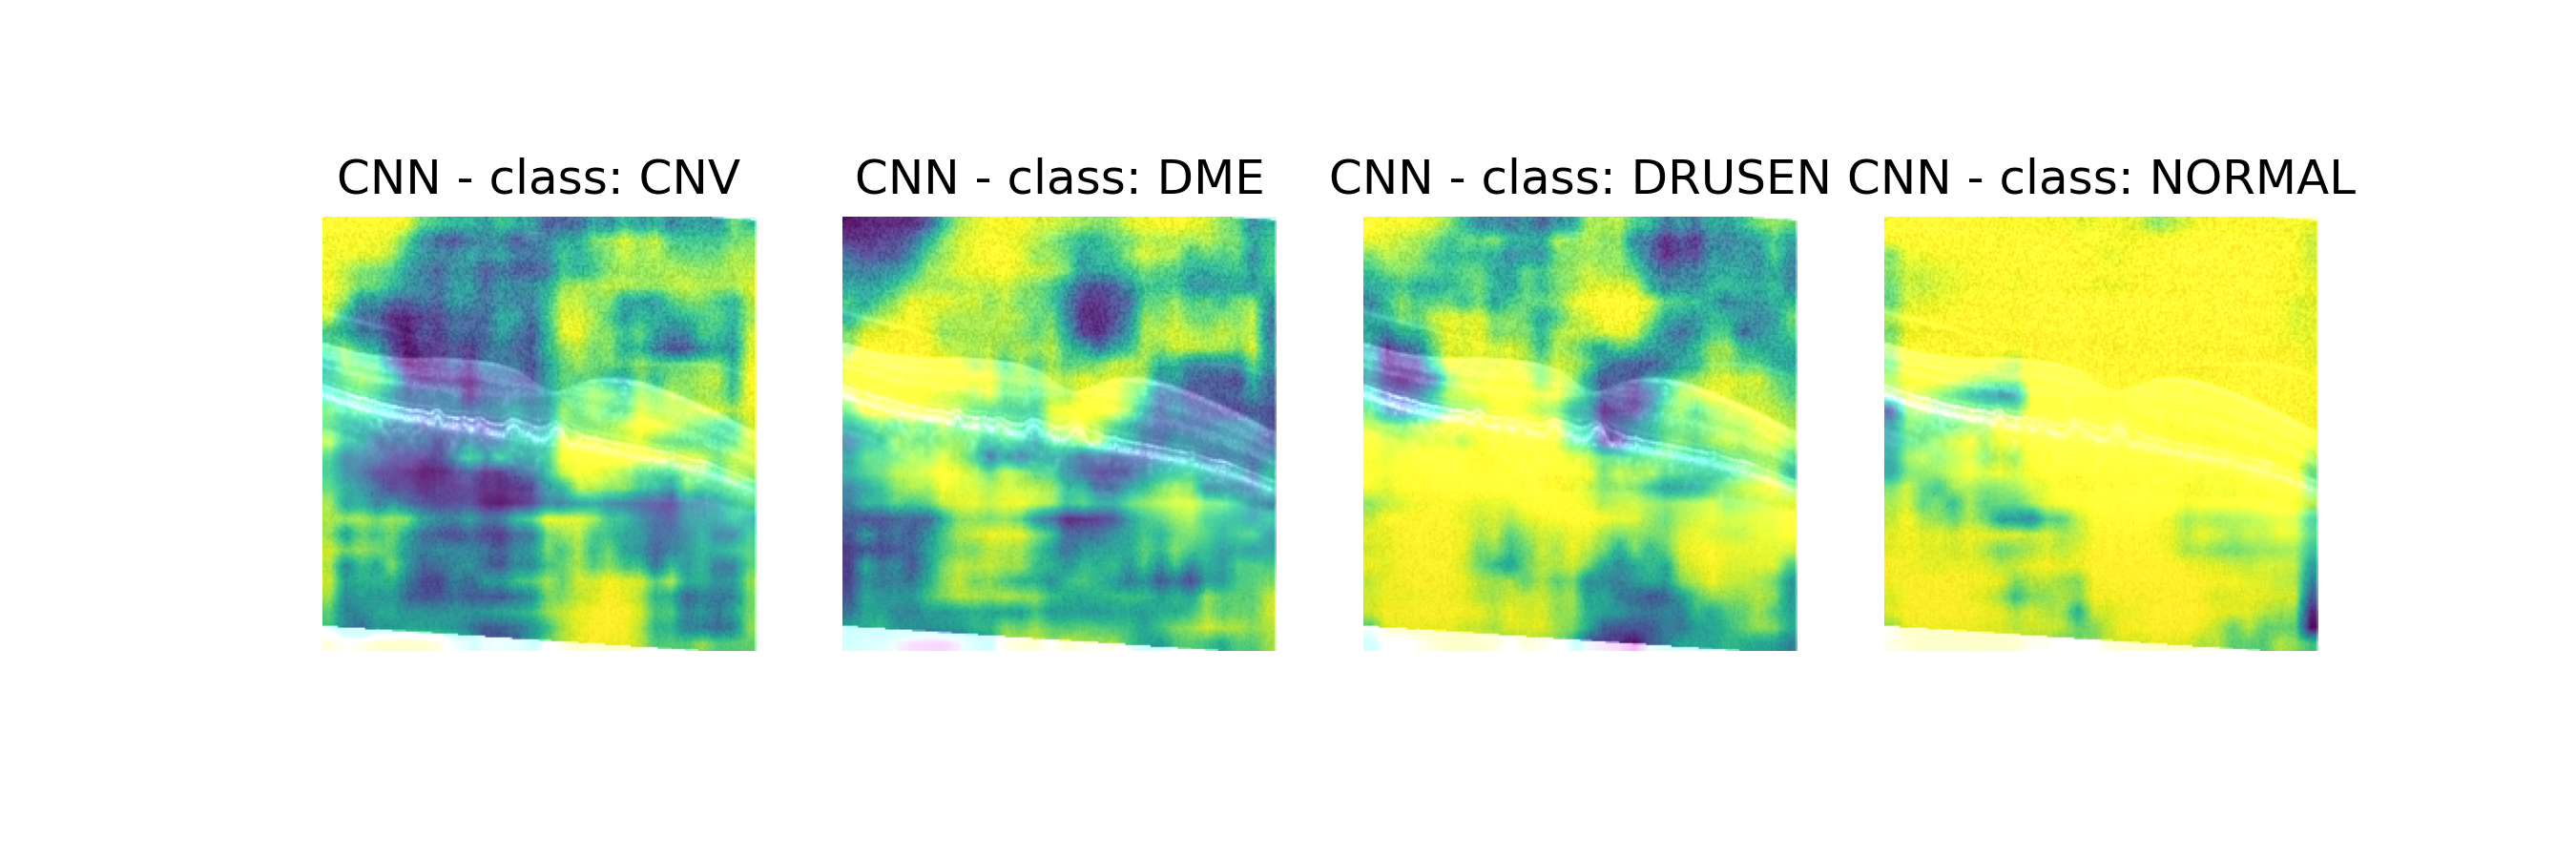
\includegraphics[width=400px]{5_occlusion_sensitivity_transfer.png}
  \caption{Transfer Model occlusion sensitivity per class.}
  \label{fig:occlusion-transfer-5}
\end{figure}


The confusion matrices for both models indicate high accuracy with minimal errors, demonstrating their effectiveness in classifying retinal images across four classes (Figures \ref{fig:confusion-matrix-cnn-5} and \ref{fig:confusion-matrix-transfer-5}). However, the transfer model's ability to start with a better loss value and its potential for improvement make it a more suitable choice for this task.

\begin{figure}[h]
  \centering
  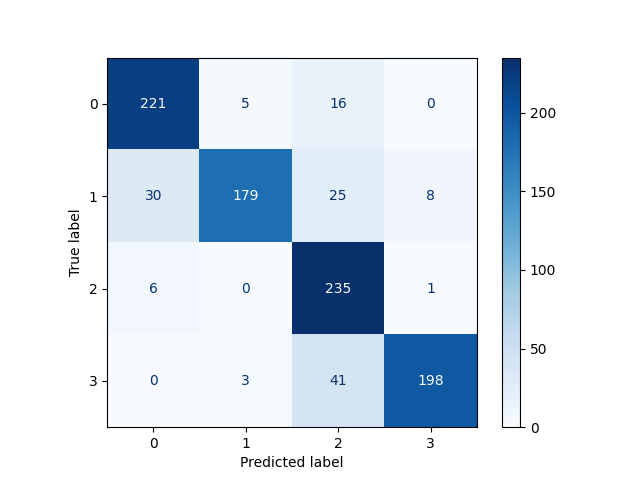
\includegraphics[width=250px]{5_confusion_matrix.png}
  \caption{Confusion matrix for simple CNN.}
  \label{fig:confusion-matrix-cnn-5}
\end{figure}


\begin{figure}[h]
  \centering
  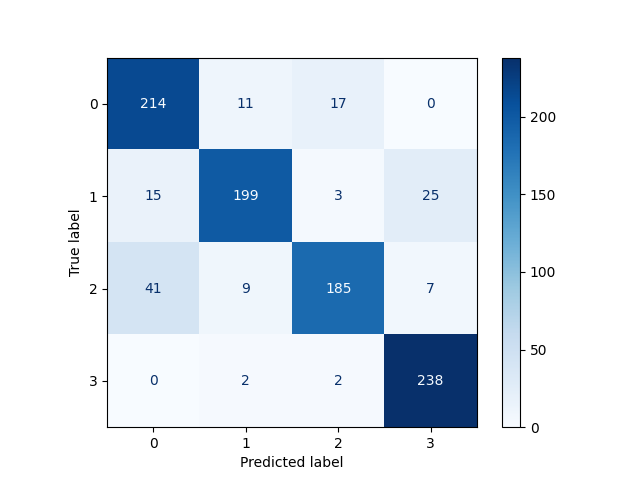
\includegraphics[width=250px]{5_confusion_matrix_transfer.png}
  \caption{Confusion matrix for transfer model.}
  \label{fig:confusion-matrix-transfer-5}
\end{figure}


In conclusion, while both the handcrafted CNN and the transfer learning model perform well in classifying retinal images to identify eye disorders, the transfer model offers a more robust starting point and greater potential for enhancement. Its ability to capture patterns and make accurate predictions with less initial loss underscores its suitability as the best model for this task. The deep neural network's capacity to classify retinal images effectively is evident, with the transfer model showing more promise for future developments in this field, making it a great tool for medical purposes of diagnosing diseases using retinal images.


% \pagebreak

% \section{References}

% \bibliographystyle{acm}
% \bibliography{refs}

\end{document}
